%! TEX program = lualatex
\documentclass[11pt]{article}
% Packages
%\usepackage[margin=1.5in]{geometry}
\usepackage{index}
\usepackage{amsbsy} % Bold math symbols
\makeindex
%\usepackage[utf8]{inputenc}
\usepackage{tcolorbox}
\tcbuselibrary{theorems}
\tcbuselibrary{skins}
\tcbuselibrary{breakable}
\usepackage{varwidth}
\usepackage{textcomp}
\usepackage{amsmath}
\usepackage{esint}
\usepackage{titlesec}
\usepackage{xcolor}
\usepackage{titling}
\usepackage[linktocpage]{hyperref}
\usepackage{pgfplots}
\usepackage{multicol}
\setlength{\columnsep}{2em}
\usepackage{caption}
\usepackage{amsthm}
\usepackage{import}
\usepackage{cancel}
\usepackage{caption}
\usepackage{nicematrix}
%\usepackage{parskip}
\usepackage{enumerate}
\usepackage{graphicx}
\usepackage[italian]{babel}
\usepackage{setspace}
\setstretch{1.2}
% To reset footnote numbering each page
\usepackage[perpage]{footmisc}
\usepackage{faktor}
\usepackage{tikz-cd}
\hypersetup{colorlinks,breaklinks, linkcolor=[RGB]{133,68,66}}
\definecolor{mastercolor}{HTML}{854442}
\definecolor{nred}{HTML}{bf0040}


% Titles 
\title{Appunti di\\ \vspace{.3cm} Analisi 3}
\author{Manuel Deodato}
\date{}




\newtheoremstyle{style}% name of the style to be used
{5pt}% measure of space to leave above the theorem. E.g.: 3pt
{5pt}% measure of space to leave below the theorem. E.g.: 3pt
{\normalfont}% name of font to use in the body of the theorem
%{15pt}% measure of space to indent
{0pt}% measure of space to indent
{\noindent\bfseries}% name of head font
{}% punctuation between head and body
{ }% space after theorem head; " " = normal interword space
{\thmname{#1}\thmnumber{ #2}{\thmnote{ (#3)}.\ }}


\theoremstyle{style}
\newtheorem{esempio}{Esempio}[section]
\newtheorem{definizione}{Definizione}[section]
\newtheorem{prop}{Proposizione}[section]
\newtheorem{teorema}{Teorema}[section]
\newtheorem{lemma}{Lemma}[teorema]
\newtheorem{corollario}{Corollario}[teorema]
\newtheorem{osservazione}{Osservazione}[section]
\newtheorem{notazione}{Notazione}[section]
\newtheorem{esercizio}{Esercizio}[section]
\newenvironment{svolgimento}{\renewcommand\qedsymbol{$\blacksquare$}\begin{proof}[Svolgimento]}{\end{proof}}




%% Generic box
\newtcolorbox{eqbox}[1][]
{
colback=gray!10,
arc=0pt,
boxrule=0pt,
title=#1
}

 \newenvironment{boxenv}[1][]{
    \begin{eqbox}[#1]
    }{
   \end{eqbox}
}



%Captions
\captionsetup[figure]{font=footnotesize,labelfont=footnotesize}
\captionsetup[table]{font=footnotesize,labelfont=footnotesize}
%Titlesec
\titleformat{\section}
{\fontsize{20}{20}\scshape}
{{\color{mastercolor}\fontsize{30}{20}\selectfont\thesection}}
{0.7em}
{}
\titlespacing*{\section}{0pt}{*2}{1cm}
\titlespacing*{\subsection}{0pt}{*5}{.25cm}
\titlespacing*{\subsubsection}{0pt}{*4.5}{.25cm}

% Personalizza la formattazione della subsection
\titleformat{\subsection}[block]{\fontsize{15}{20}\bfseries}{\thesubsection}{.5em}{}


% Personalizza la formattazione della subsubsection
\titleformat{\subsubsection}[block]{\fontsize{13}{10}\bfseries}{\thesubsubsection}{.5em}{}

% Maketitle customization
\renewcommand{\maketitle}{
\begin{center}
{\sffamily
{\fontsize{20}{20}\selectfont\MakeUppercase{\thetitle}}}

\vspace{0.2in}

{\large\MakeUppercase{\theauthor}}
\end{center}
}

%Evaluate symbol
\DeclareMathOperator{\di}{d\!}
\newcommand*\Eval[3]{\left.#1\right\rvert_{#2}^{#3}}

%%%%%%% Numero delle equazioni in formato a.b
\numberwithin{equation}{subsection}
%%%%%

%%%%%%%%%% Personalizzazione numeri lista
\renewcommand{\theenumi}{(\arabic{enumi})}

%%%% Table of contents

\usepackage[titles]{tocloft}

\renewcommand{\cftdot}{}
\usepackage{titletoc}
%\setcounter{tocdepth}{2}

%%%%%%%%%%%%%%%% Toc style

% Personalizzazione scritta indice


% Font
\renewcommand{\textbf}[1]{\textsf{\bfseries #1}}
\usepackage{fontspec}
\usepackage{unicode-math}
\usepackage[default]{fontsetup}



%%% Hook
\newcommand{\longhookrightarrow}{\lhook\joinrel\longrightarrow}


\begin{document}
\maketitle
\vspace{5cm}
\begin{center}
		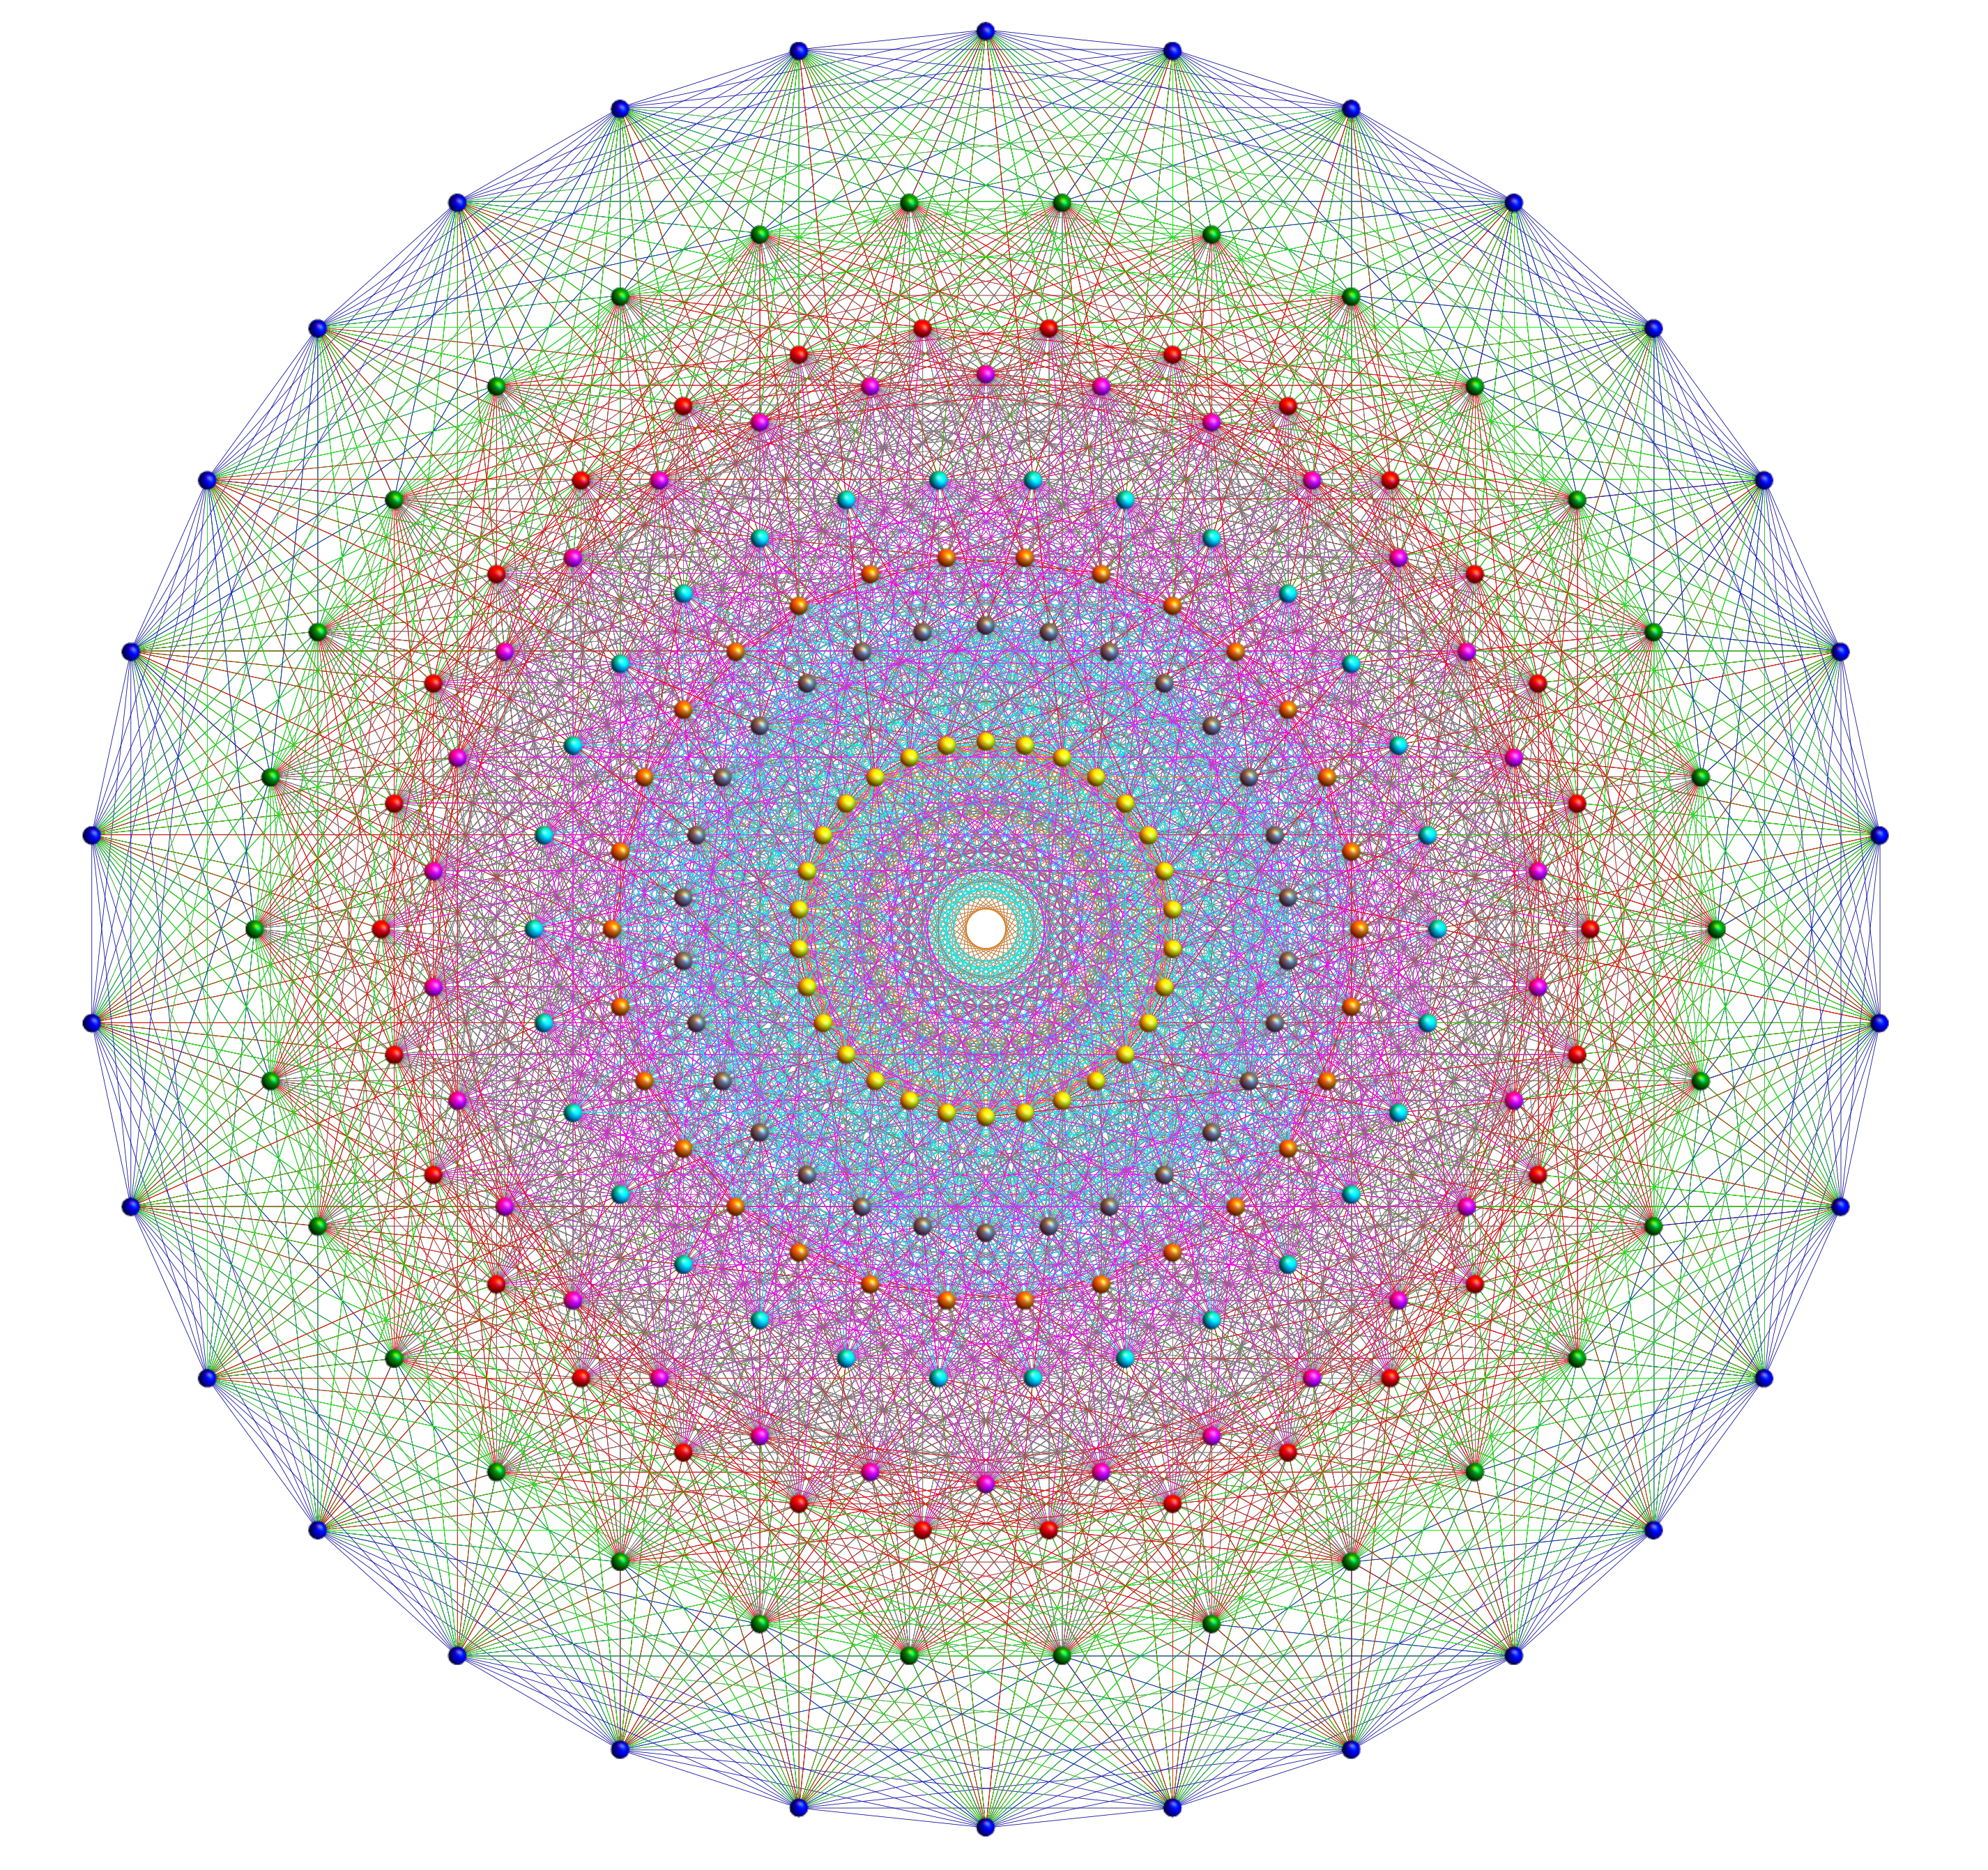
\includegraphics[width=.9\columnwidth]{front.jpg}
\end{center}
\newpage
\tableofcontents
\newpage
\section{Teoria della misura}
\subsection{Introduzione}
	L'obiettivo \`e arrivare a costruire una funzione che permetta di misurare i sottoinsiemi di $\mathbb{R}^d$, o quantomeno la maggior parte, e una conseguente teoria dell'integrazione che abbia un buon comportamento rispetto al passaggio al limite.

	Per ottenere il volume di generici sottoinsiemi di $\mathbb{R}^d$ \`e opportuno partire da oggetti la cui geometria sia nota e \textit{rivestire} tali sottoinsiemi con questi oggetti in modo tale da approssimarne arbitrariamente bene la misura.
	A questo scopo, si definisce il seguente oggetto fondamentale.
	\begin{definizione}
		[Plurintervallo]
	Si definisce \textit{plurintervallo} un sottoinsieme di $I \subseteq \mathbb{R}^d$ tale per cui esistono degli intervalli $I_k \subseteq \mathbb{R}$ tali che
	\[
	I = \prod_{k=1} ^d I_k
	\] 
	dove il prodotto \`e il prodotto cartesiano.
	In altri termini, un plurintervallo $I$ \`e della forma
	\[
	I = \prod_{k=1} ^d (a_k,b_k)
	\] 
	con $-\infty < a_k < b_k <+\infty, \ \forall k$.
	\end{definizione}
	\begin{osservazione}
	Fondamentalmente, un plurintervallo \`e un rettangolo per $d=2$, un parallelepipedo per $d=3$, eccetera.
	\end{osservazione}
	La geometria di questi oggetti \`e nota perch\'e la loro misura\footnote{Cio\`e il loro volume per $d=3$, la loro area per $d=2$, eccetera.} \`e nota ed \`e data da:
	\[
	\lvert I \rvert  = \prod_{k=1} ^d (b_k - a_k) = \prod_{k=1} ^d \lvert I_k \rvert 
	\] 
	\subsection{Misura esterna}
	Per definire una misura, si parte col definire una misura esterna, cio\`e una funzione $\mu^*  : \mathcal{P} (\mathbb{R}^d) \to [0,+\infty]$ tale che
	\begin{enumerate}[(a).]
		\item $\mu^* (\varnothing)=0$;
		\item se $A \subseteq B \subseteq \mathbb{R}^d$, allora $\mu^* (A) \le \mu^* (B)$;
		\item data $\left\{ E_i \right\} _{i=1} ^{+\infty} $ famiglia numerabile di insiemi, vale
			\[
			\mu^* \left(\bigcup_{i=1} ^{+\infty} E_i\right) \le \sum_{i=1}^{+\infty} \mu^* (E_i)
			\] 
	\end{enumerate}
	Inoltre, si richiede che se $I \subseteq \mathbb{R}^d$ \`e un plurintervallo, allora $\mu^* (I) = \lvert I \rvert $.
	Si d\`a, allora, la seguente definizione e se ne verificano le propriet\`a.
	\begin{definizione}
		[Misura esterna di Lebesgue]
	Sia $E \subseteq \mathbb{R}^d$ e sia $S$ un suo ricoprimento, tale che
	\[
	E \subseteq \bigcup_{k=1} ^{+\infty} I_k
	\] 
	con $I_k \subseteq \mathbb{R}^d$ plurintervalli. Sia, inoltre
	\[
	\sigma (S) = \sum_{k=1}^{+\infty} \lvert I_k \rvert 
	\] 
	il volume totale\footnote{Cio\`e si conta anche il volume condiviso tra pi\`u plurintervalli.} del ricoprimento; allora si definisce la \textit{misura esterna} di $E$ come:
	\[
	\mu^* (E) := \inf_S \sigma 
	\] 
	\end{definizione}
Ai fini della teoria, si assume che la frontiera degli insiemi sia a misura nulla, cio\`e si dice che due plurintervalli $I_k, I_j \subseteq \mathbb{R}^d$ \textit{non sono sovrapposti} se
\[
	\mathring{I}_k \cap \mathring{I}_j = \varnothing, \ \text{ per } k \neq j
\] 
\begin{teorema}
	Sia $I \subseteq \mathbb{R}^d$ un plurintervallo; allora $\mu^* (I) = \lvert I \rvert $.
\end{teorema}
	\begin{proof}
		Evidentemente $I$ \`e il pi\`u piccolo ricoprimento di se stesso che, quindi, minimizza $\sigma (S)$, pertanto, per definizione, si ha $\mu^* (I) = \lvert I \rvert $.
	\end{proof}
\begin{teorema}
	Siano $A,B \subseteq \mathbb{R}^d$ tali che $A \subseteq B$; allora $\mu^* (A) \le \mu^* (B)$.
\end{teorema}
	\begin{proof}
		Applicando direttamente la definizione, si nota che:
		\[
		\mu^* (A) = \inf_{S_A} \sigma (S_A) \le \inf_{S_B} \sigma (S_B) = \mu^* (B)  
		\] 
		visto che ogni ricoprimento $S_B$ di $B$ ricopre anche $A$.
	\end{proof}
\begin{corollario}
	Siano $E \subseteq E' \subseteq \mathbb{R}^d$, con $\mu^* (E') = 0$; $\mu^* (E) = 0$.
\end{corollario}
\begin{teorema}\label{thfond}
	Sia $E \subseteq \mathbb{R}^d$; allora $\forall \varepsilon >0, \ \exists G \subseteq \mathbb{R}^d$ aperto tale che $E \subset G$ e $\mu^* (G) < \mu^* (E) + \varepsilon $.
\end{teorema}
\begin{proof}
	Sia $\left\{ I_k \right\} _{k=1} ^{+\infty} $ una famiglia numerabile di plurintervalli chiusi di $\mathbb{R}^d$ tali che
	\[
	E \subset \bigcup _{k=1} ^{+\infty}I_k \hspace{1cm} \sum_{k=1}^{+\infty}\lvert I_k \rvert  \le \mu^* (E) + \varepsilon  
	\] 
	Allora si costruiscono dei nuovi intervalli $I_k^*$ tali che $I_k \subset \mathring{I}_k^*$ e $\lvert I_k^* \rvert \le \lvert I_k \rvert + \varepsilon / 2^{k} $; allora il relativo insieme $G$ aperto \`e dato da
	\[
		G = \bigcup_{k=1} ^{+\infty} \mathring{I}_k^*
	\] 
	Infatti
	\[
	\mu^* (G) = \sum_{k=1}^{+\infty} \lvert I_k^* \rvert \le  \sum_{k=1}^{+\infty}\left( \lvert I_k \rvert + \frac{\varepsilon }{2^{k} }\right) \le \mu^* (E)+\varepsilon 
	\] 
	
\end{proof}
\begin{osservazione}
Relativamente al teorema precedente, si notano due cose: intanto fa uso della topologia di $\mathbb{R}^d$ e poi afferma che un generico insieme $E \subseteq \mathbb{R}^d$ \`e approssimabile arbitrariamente bene tramite un aperto $G$.
\end{osservazione}

\begin{teorema}
	Sia $E \subseteq \mathbb{R}^d$; allora $\exists H = \bigcap_{j=1} ^{+\infty} G_j$, con $G_j$ aperti, tale che $E \subset H$ e $\mu ^*(E) = \mu ^*(H)$.
\end{teorema}
	\begin{proof}
		Dalla definizione di misura esterna di $E$, si sa che
		\[
		\mu ^*(E) = \inf \left\{ \mu ^*(F)  \mid F \text{ aperto e } E \subseteq F \right\} 
		\] 
		Di conseguenza, per definizione di estremo inferiore, devono esistere degli aperti $G_n \supseteq E$ tali per cui
		\[
		\mu ^*(G_n) < \mu ^*(E) + \frac{1}{n}
		\] 
		con $n \in \mathbb{N}$.
		Allora si vede che, preso 
		\[
		H = \bigcap _{n=1} ^{+\infty} G_n 
	\]
	si ha $E \subset H$ perch\'e ogni $G_n$ contiene $E$, quindi $\mu ^*(H)\ge \mu ^*(E)$, ma, allo stesso tempo
	\[
	\mu ^*(H)\le \mu ^*(E) + \frac{1}{n}, \ \forall n
	\] 
	quindi, passando al limite per $n\to +\infty$, si rimane con la disuguaglianza
	\[
	\mu ^*(E) \le \mu^* (H) \le \mu ^*(E)
	\] 
	da cui $\mu^* (H) = \mu ^*(E)$.
\end{proof}
Gli insiemi che sono intersezione numerabile di aperti sono detti $G_\delta $, mentre quelli che sono unione numerabile di chiusi sono detti $F_\sigma $; in questo caso, l'$H$ del teorema \`e un $G_\delta $.
\begin{teorema}
	Se $\left\{ E_n \right\} _{n\in \mathbb{N}} \subseteq \mathbb{R}^d$, allora
	\[
	\mu ^*\left(\bigcup_{n=1}^{+\infty} E_n \right) \le \sum_{n=1}^{+\infty} \mu ^*(E_n)
	\] 
\end{teorema}
\begin{proof}
	Se la somma diverge, la tesi \`e verificata, quindi si assume che $\sum_{n}^{} \mu ^*(E_n)<+\infty$.
Visto che $\mu ^*(E_n)$ \`e definita come l'estremo inferiore sulla somma delle misure dei plurintervalli di un ricoprimento, $\forall \varepsilon >0$ si pu\`o trovare un ricoprimento $\left\{ Q_{n,k}  \right\} _{k\in \mathbb{N}} $ di $E_n$ tale che
\[
\sum_{k=1}^{+\infty} \lvert Q_{n,k}  \rvert \le \mu ^*(E_n) + \frac{\varepsilon }{2^n}
\] 
Visto che l'unione di questi ricoprimenti al variare di $n$ forma un ricoprimento anche di $\bigcup_{n\in \mathbb{N}} E_n$, allora
\[
\mu ^*\left(\bigcup_{n=1} ^{+\infty} E_n\right) \le \sum_{n=1}^{+\infty} \sum_{k=1}^{+\infty} \lvert Q_{n,k}  \rvert \le \sum_{n=1}^{+\infty}\left( \mu ^*(E_n) + \frac{\varepsilon }{2^n}\right) = \sum_{n=1}^{+\infty} \mu ^*(E_n) + \varepsilon 
\] 
Per l'arbitrariet\`a di $\varepsilon $, si ha la tesi.
\end{proof}
\begin{lemma}
	Siano $E_1, E_2\subseteq \mathbb{R}^d$ tali che $d(E_1,E_2) > 0$, con
	\[
	d(E_1,E_2) = \inf_{\substack{x \in E_1 \\ y \in E_2}} d(x,y) 
	\] 
	Allora $\mu ^*(E_1\cup E_2) = \mu ^*(E_1) + \mu ^*(E_2)$.
\end{lemma}
	\begin{proof}
		Per la propriet\`a di sub-additivit\`a della misura esterna, la disuguaglianza $\mu ^*(E_1\cup E_2) \le \mu ^*(E_1) + \mu ^*(E_2)$ \`e gi\`a verificata, quindi si verifica la disuguaglianza inversa.
		Sia $\delta = d(E_1,E_2)$ e sia $\left\{ Q_k \right\} _{k \in \mathbb{N}} $ una famiglia di plurintervalli di $\mathbb{R}^d$ che ricopre $E_1\cup E_2$, con 
		\[
			\sum_{k=1}^{+\infty} \lvert Q_k \rvert \le \mu ^*(E_1\cup E_2) + \varepsilon 
		\] 
		Si pu\`o spezzare ciascun plurintervallo $Q_k$ in sotto-plurintervalli $Q_{k,n} $ di diametro $\delta / 2$. La loro unione ricostruire ciascun $Q_k$ e, quindi, ricopre $E_1\cup E_2$:
		\[
		Q_k = \bigcup_{n} Q_{k,n} \hspace{1cm} E_1 \cup E_2 \subset \bigcup_{k=1} ^{+\infty}Q_k = \bigcup_{k=1} ^{+\infty} \bigcup_{n} Q_{k,n} 
	\] 
	Si indica questo nuovo ricoprimento con $\left\{ Q'_k \right\} _{k \in \mathbb{N}} $ e soddisfa
	\[
	\sum_{k=1}^{+\infty} \lvert Q'_k \rvert =\sum_{k=1}^{+\infty} \lvert Q_k \rvert \le \mu ^*(E_1\cup E_2) + \varepsilon 
	\] 
con il vantaggio che ogni $Q'_k$ \`e spesso $\delta / 2$.
Questo significa che la somma $\sum_{}^{} \lvert Q'_k \rvert $ si pu\`o spezzare nel volume che contiene punti di $E_1$ e nel volume che contiene punti di $E_2$; chiaramente non ci potr\`a essere alcun $Q'_k$ che contenga punti di entrambi per la condizione sullo spessore.
Cos\`i facendo, si nota che:
\[
\sum_{k=1}^{+\infty} \lvert Q'_k \rvert = \sum_{i : Q'_i\cap E_1 \neq \varnothing}^{} \lvert Q'_i \rvert + \sum_{i : Q'_i \cap E_2\neq \varnothing}^{} \lvert Q'_i \rvert \ge \mu ^*(E_1) + \mu ^*(E_2)
\] 
Unendo le disuguaglianze, si trova che
\[
\mu ^*(E_1) + \mu ^*(E_2) \le \mu ^*(E_1\cup E_2) + \varepsilon 
\] 
Visto che $\varepsilon $ \`e arbitrario, allora si ottiene che $\mu ^*(E_1) + \mu ^*(E_2) \le \mu ^*(E_1\cup E_2)$ che, insieme alla disuguaglianza opposta trovata prima, permette di concludere l'uguaglianza e, quindi, la tesi.
	\end{proof}
\subsection{Misurabilit\`a}
La misura esterna \`e definita su tutti i possibili sottoinsiemi di $\mathbb{R}^d$, cio\`e $\mu ^* : \mathcal{P} (\mathbb{R}^d) \to [0,+\infty]$; adesso si introduce il concetto di misurabilit\`a e la nuova funzione misura sar\`a definita sulla classe degli insiemi misurabili di $\mathbb{R}^d$.
\begin{definizione}
	[Insieme misurabile]
	Sia $E \subseteq \mathbb{R}^d$; si dice che $E$ \`e \textit{misurabile} se $\forall \varepsilon >0$, si trova un $G \subseteq \mathbb{R}^d$ aperto, con $E \subset G$, tale che $\mu ^*(G \setminus E) < \varepsilon $.
\end{definizione}
Per definizione, se $E \subseteq \mathbb{R}^d$ \`e misurabile, allora la sua misura \`e definita da:
\[
\mu (E) := \mu ^*(E)
\] 
dove $\mu:\mathscr{L} \to [0,+\infty] $ \`e definita sulla classe degli insiemi misurabili secondo Lebesgue, indicata con $\mathscr{L} \subseteq \mathcal{P} (\mathbb{R}^d)$.
Da questa definizione, discendono le seguenti propriet\`a.
\begin{prop}
	Se $A \subseteq \mathbb{R}^d$ \`e un aperto, allora $A$ \`e misurabile.
\end{prop}
	\begin{proof}
		Per definizione diretta di misurabilit\`a, si pu\`o prendere proprio $A$ come aperto, per cui $\mu ^*(A \setminus A) = \mu ^* (\varnothing)=0 < \varepsilon , \ \forall \varepsilon >0$.
	\end{proof}
\begin{prop}
	Se $E \subseteq \mathbb{R}^d$ tale che $\mu ^*(E) = 0$, allora $E$ \`e misurabile.
\end{prop}
	\begin{proof}
		Per il teorema \ref{thfond}, $\forall \varepsilon >0$, si pu\`o prendere un aperto $G \supseteq E$ tale che $\mu ^*(G) \le \mu ^*(E) + \varepsilon = \varepsilon $, quindi $\mu ^*(G\setminus E) \le \mu ^*(G) < \varepsilon $, quindi $E$ \`e misurabile.
	\end{proof}
Si nota che la propriet\`a di misurabilit\`a di insieme \`e nettamente pi\`u forte del teorema \ref{thfond}; infatti, se $E \subseteq \mathbb{R}^d$ e $G \supset E$ \`e un aperto tale che $\mu ^*(G) < \mu ^*(E) + \varepsilon $, allora si nota che 
\[
G = E \cup (G\setminus E) \implies \mu ^*(G) \le \mu ^*(E) + \mu ^*(G\setminus E)
\] 
cio\`e non \`e possibile dedurre che $\mu ^*(G\setminus E) < \varepsilon $ dal fatto che $\mu ^*(G) <\mu ^*(E) + \varepsilon $.
\begin{lemma}
	Siano $\left\{ I_k \right\} _{k=1} ^{+\infty} $ dei plurintervalli di $\mathbb{R}^d$ tali che $\mathring{I}_k \cap \mathring{I}_j = 0, \ k\neq j$; allora $\bigcup_k I_k$ \`e misurabile e 
	\[
 \left\lvert \bigcup_{k=1} ^{+\infty} I_k \right\rvert = \sum_{k=1}^{+\infty} \lvert I_k \rvert 
	\] 
\end{lemma}
\begin{teorema}
	La classe degli insiemi misurabili $\mathscr{L} \subset \mathbb{R}^d$ \`e una $\sigma $-algebra.
\end{teorema}
\begin{teorema}
	Se $\left\{ E_k \right\} _{k=1} ^{+\infty} \subseteq \mathbb{R}^d$ \`e una famiglia di insiemi misurabili, allora $\bigcup_k E_k$ \`e misurabile.
\end{teorema}
\begin{teorema}
	Se $F\subseteq \mathbb{R}^d$ \`e chiuso, allora \`e misurabile.
\end{teorema}
\begin{teorema}
	Se $I$ \`e un plurintervallo chiuso, si ha $\mu (\partial I) = 0$.
\end{teorema}





\end{document}
